\section{Central forces}
A force \( F(x,y,z) \) is called central if it has the form:
\[ 
  \textbf{F} = F(r)\hat{ \textbf{r}} = \frac{F(r)}{r} \textbf{r}
\]
where \( \textbf{r} = x\hat{i} + y \hat{j} + z \hat{k} \) and \( r = \sqrt{x^2
+ y^2 + z^2} = (x^2 + y^2 + z^2)^{\frac{1}{2}}\)
Central forces act towards or away from the origin. The maginitude is dependant
on the distance from the origin.
\\\\
Consider the gradient of the radial distance,
\begin{align*} 
  \nabla r &= \Bigg ( \frac{\partial{r}}{\partial{x}},
  \frac{\partial{r}}{\partial{y}}, \frac{\partial{r}}{\partial{z}}\Bigg) \\
	   &= (x^2 + y^2 + z^2)^{\frac{1}{2}} (x,y,z)\\
	   &= \frac{1}{r} \; \underline{r} = \underline{ \hat{r}}
\end{align*}
Let \( F(r) = -\displaystyle \frac{dV}{dr} \) for some function \( V \). We
show that the central force \( \textbf{F}(r) = F(r) \hat{r} \) is conserved
with potential function \( V(r) \).
\begin{proof}

\begin{align*}
  - \nabla V  &= \Bigg(- \frac{\partial{V}}{\partial{x}},
  - \frac{\partial{V}}{\partial{y}}, - \frac{\partial{V}}{\partial{z}}\Bigg)\\
  &= \Bigg(- \frac{dV}{dr} \frac{\partial{r}}{\partial{x}}, - \frac{dV}{dr}
    \frac{\partial{r}}{\partial{y}}, - \frac{dV}{dr}
  \frac{\partial{r}}{\partial{z}}\Bigg) \;\; (\text{By the chain rule}) \\
  &= F(r) \Bigg( \frac{\partial{r}}{\partial{x}},
  \frac{\partial{r}}{\partial{y}}, \frac{\partial{r}}{\partial{z}}\Bigg)
  = F(r) \hat{r}\\
  \frac{dE}{dt} &= \frac{1}{2}m \underline{ \dot{v}} \cdot \underline{v}
+ \frac{1}{2} m \underline{v} \cdot \underline{ \dot{v}} + \frac{dV}{dr}
\dot{r} = m \underline{a} \cdot \underline{v} + \frac{dV}{dr} \dot{r} 
\end{align*}
Therefore all \textbf{central forces are conservative} (provided that \(
\textbf{F}(r) \) is integrable). Hence a particle moving in a central force \(
\textbf{F}(r) = -V'(r) \hat{r}\) has energy
\[ 
  E = \frac{1}{2} mv^2 + V(r)
\]
which remains constant.
\end{proof}
\section{Angular Momentum}
A particle with mass \( m \), velocity \( \textbf{v} \) and position \(
\textbf{r} \), then the angular momentum is given by
\[ 
  L = m( \textbf{r} \times \textbf{v} )
\]
A force exerted on the particle, by Newton's Second Law.
\begin{align*}
  \underline{\dot{L}} &= m( \underline{\dot{\textbf{r}}} \times
  \underline{\textbf{v}}) + m( \underline{ \textbf{r}} \times \underline{ \dot{
  \textbf{v}}}) \\
  &= m ( \underline{ \textbf{v}} \times \underline{ \textbf{v}}) + m(
  \underline{ \textbf{r}} \times \underline{ \textbf{a}})\\
  &= \underline{ \textbf{r}} \times \underline{ \textbf{F}}
\end{align*}
We call \( \textbf{r} \times \textbf{F} \) the \textbf{torque} for a central
force \( \textbf{F} = \displaystyle \frac{F(r)}{r} \textbf{r} \). So the time
derivative is 
\begin{align*}
  \underline{ \dot{ \textbf{L}}} = \textbf{ \underline{r}} \times \underline{
  \textbf{F}} &= \frac{F(r)}{r} ( \underline{ \textbf{r}} \times \underline{
\textbf{ r}}\\
  &= 0
\end{align*}
As \( \textbf{L} \) is constant (it's not gonna change anytime soon), we have
\textbf{conservation of angular momentum}. Also as angular momentum is a vector
quantity \( \implies \) that both the magnitude and direction is constant as
well.
\\\\
\textbf{By the definition of the cross product, the direction of the angular
momentum is perpendicular to the position and velocity vectors.}
\\\\
This means that motion is confined to a plane. \textbf{Without any loss of
generality}, we can choose this plane to be the \( x-y \) plane.
\section{Polar Coordinates}
Its natural to represent central force problems in polar coordinates in \(
\mathbb{R}^2 \). These are an example of \textbf{curvlinear coordinates}. The
basic vectors used in curvlinear coordinates are \textbf{not} fixed in space.
They change according to a position of a particle. 
\begin{example}
One basis vector is given by
\[
  \hat{ \textbf{r}} = \cos(\theta) \hat{i} + \sin(\theta) \hat{j}
\]
We can check that a perpendicular unit vector is given by
\[ 
  \hat{\theta} = - \sin(\theta) \hat{i} + \cos(\theta) \hat{j}
\]
The vectors \( \underline{ \textbf{r}} \) provide an orthogonal basis for \(
\mathbb{R} ^2 \). We need to to check if the following two properties hold
\begin{enumerate}
  \item \[\frac{d \hat{r}}{d\theta} = \hat{\theta}\]
  \item \[\frac{d \hat{\theta}}{d\theta} = -\hat{r}\]
\end{enumerate}

We can obtain the following expressions for the velocity and acceleration

\begin{align*}
  \underline{r} &= r \underline{ \hat{r}}\\
  \underline{v} = \underline{ \dot{r}} &= \dot{r} \underline{ \hat{r}}
  + r \frac{d \underline{ \hat{r}}}{dt}\\
  &= \dot{r} \underline{ \hat{r}} + r \frac{d \hat{r}}{d\theta}
  \frac{d\theta}{dt}\\
  &= \dot{r} \underline{ \hat{r}} + r \dot{\theta} \underline{ \hat{ \theta}}
\end{align*}
For the acceleration
\begin{align*}
  \underline{a} &= \frac{d \underline{v}}{dt}\\
  &= \ddot{r} \underline{ \hat{r}} + \dot{r} \frac{d \underline{ \hat{r}}}{dt}
  + \dot{r} \dot{\theta} \hat{\theta} + r \ddot{\theta} \hat{\theta}
  + r \dot{\theta} \frac{d \hat{\theta}}{dt}\\
  &= \ddot{r} \underline{ \hat{r}} + \dot{r} \frac{d \underline{
  \hat{r}}}{d\theta} \dot{\theta} + \dot{r} \dot{\theta} \hat{\theta}
  + r \ddot{\theta} \underline{ \hat{\theta}} + r \dot{\theta} \frac{d
  \underline{ \hat{\theta}}}{d\theta} \dot{\theta}\\
  &= ( \ddot{r} - r \dot{\theta}^2) \underline{ \hat{r}} + (2 \dot{r}
  \dot{\theta} + r \ddot{\theta}) \underline{\hat{\theta}}  
\end{align*}
We are dealing with a central force \( \textbf{F} = -V'(r) \hat{r} \) such that
the equation of motion is
\[ 
  -V'(r) \hat{r} = m( \ddot{r} - r \dot{ \theta}^2) \hat{r} + m(2 \dot{r}
  \dot{\theta} + r \ddot{\theta}) \hat{\theta}
\]
Equating the radial and angular components. For the radial part.
\[ 
  \ddot{r} - r \dot{\theta}^2 = - \frac{V'(r)}{m}
\]
And for the angular equation
\[ 
  2 \dot{r} \dot{\theta} + r \ddot{\theta} = 0;
\]
Rewriting the angular equation we have
\[ 
  \frac{d}{dt}(r^2 \dot{\theta}) = 0
\]
This is saying that the magnitude of angular momentum is constant over time.
I.e 
\[ 
  L = mr^2 \dot{theta}
\]
Where \( L \) is constant. We can describe the motion of the particle by the
radial equation
\[ 
  \ddot{r} = \frac{L^2}{m^2r^3} - \frac{V'(r)}{m}
\]
\end{example}
\section{Circular Motion}
Attractive central forces are capable of producing circular motion moving at
constant speed. Given for circular motion, \( r \) is constant \( \implies
\dot{r} = \ddot{r} = 0 \). We have
\begin{align*}
  v^2 &= ( \dot{r} \underline{\hat{r}} + r \dot{\theta}
  \underline{\hat{\theta}})\cdot( \dot{r} \underline{\hat{r}} + r \dot{\theta}
  \underline{\hat{\theta}})\\
      &= \dot{r}^2 + r^2 \dot{\theta}^2\\
      &= r^2 \dot{\theta}^2 = \frac{L^2}{mr^2}
\end{align*}
The value of \( L \) is given by the explicit knowledge of the potential. Since
\( \ddot{r} = 0 \),
\begin{align*} 
  0 &= \frac{L^2}{m^2r^3} - \frac{V'(r)}{m}\\
  L^2 &= mr^3V'(r)  
\end{align*}
Which gives \( v^2 = \displaystyle \frac{rV'(r)}{m}\)
\begin{example}[A rotation spring without damping]
Consider a spring of length \( l  \) and spring constant \( k \), with a mass
attached at one end and fixed at the origin. The system sits on a frictionless
table and is able to rotate about the origin in the horizontal plane. This is
a central force problem where
\[ 
  F(r) = -k(r-l) \;\;\;\; V(r) = \frac{k}{2}(r-l)^2
\]

\begin{figure}[h!]
  \centering
  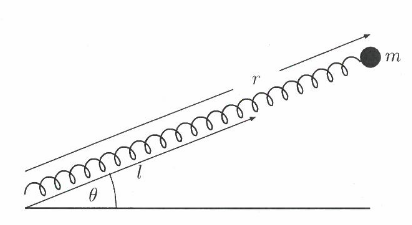
\includegraphics[width=0.4\linewidth]{./lectures/fig.png}
\end{figure}
For \( r > l \), circular motion occurs with \( \dot{r} = 0 \) and \(
v = \displaystyle \sqrt{\frac{kr(r-l)}{m}} \). Otherwise the motion is
determined by the solution to the ODE.
\[ 
  \dot{r} = \frac{L^2}{m^2r^3} - \frac{k(r-l)}{m}
\]
\end{example}
\section{The envelope of a family of functions}

Consider a function of two variables \( f(x,t) \), we can intepret this
funcition as a family of one variable functions by setting
\[ 
  y^{(t)}(x) = f(x,t)
\]
\\\\
...
\\\\
How does the concept of the envelope arises in economic modelling? Suppose that
a bakery's weekly bread roll production is described by \( f(x) \) (given the
conditions for \( x \leq 0 \) that \( f(0) = 0, f(x) \leq 0 \), \( f'(x) > 0 \)
and the cost of one kg of flour be \( c \), the selling price for one kilogram
of bread rolls is \( p \). We will consider \( p \) to be a variable, while \(
c\) is a constant. The profit \( P(p,x) \) is given by
\[ 
  P(p,x) = pf(x) - cx
\]
It is straightfoward to verify that the cross section of \( P(p,x) \) in \(
p  \)havve a local maximum when
\[ 
  f'(x) = cp^{-1}
\]
Specifically
\begin{align}
  P_x(p,x) &= pf'(x) - c\\
  P_{xx}(p,x) &= pf''(x)
\end{align}
When \( f'(x) = cp^{-1} \), Eq. (3.1) shows that a cross-section of \( P \) in
\( p \) has a critical point. Also since, \( f''(x) < 0 \), Eq. (3.2) shows
that the critical point is al local maximum.
\\\\
Let \( x = g(p) \) be the solution for (3). We define the maximised profit
function \( f^{max} \) by 
\[ 
  f^{max}(p) = pf(g(p)) - cg(p)
\]
This is the envelope of \( P(p,x) \) with the property
\[ 
  \frac{dp^{max}}{dp} = f(g(p))
\]

\begin{enumerate}
  \item \( f(x) = 4x^{1/2} \)
  \item \( f(x) = \frac{x}{x+1} \)
\end{enumerate}

both of which satisfy the required conditions for \( x \leq 0 \mid f(0) = 0,
f(x) \leq 0, \; f'(x) > 0 \) \( f''(x) < 0 \).

\begin{align*}
  f(x) &= 4x^{ \frac{1}{2} }\\
  f'(x) &= 2x^{-\frac{1}{2}} = cp^{-1} \implies x = g(p) = \frac{4p^2}{c^2}\\
  f(g(p)) &= 4 \sqrt{ \frac{4p^2}{c^2}} = \frac{8p}{c}\\
  \intertext{Then}
  p^{max} (p) &= \frac{8p}{c} \times p - c \Big( \frac{4p^2}{c^2}\Big )
  = \frac{4p^2}{c}
\end{align*}





